\section{Pianificazione}
La pianificazione di progetto è stata costruita sulla base delle scadenze presentate nella sezione §1.6 di questo documento.
Lo sviluppo del progetto è stato suddiviso nelle seguenti fasi:
\begin{itemize}
    \item Analisi;
    \item Progettazione architetturale;
    \item Progettazione di dettaglio e codifica;
    \item \glo{Validazione} e collaudo.
\end{itemize}
Ogni fase è suddivisa in attività a cui vengono associate le risorse disponibili.
    
    \subsection{Analisi}
    \textbf{Periodo}: dal 04-03-2019 al 19-04-2019. \newline
    Inizia con la formazione del gruppo e termina con la scadenza di consegna della RR.
    Questa fase si scompone in tre periodi.
        \subsubsection{Periodo analisi 1}
            \begin{itemize}
                \item Ricerca sulle tecnologie: scelta di strumenti per la comunicazione e di stesura dei documenti;
                \item Normazione: definizione di regole per la documentazione;
                \item Pianificazione: definizione delle attività preliminari per la prima fase;
                \item Scelta \glo{capitolato}: studio dei capitolati e scelta del capitolato da sviluppare. Attività bloccante per \doc{\docNameAdR{}};
                \item Verifica: alla fine delle attività precedenti vengono verificati i documenti di supporto prodotti durante questo periodo.
            \end{itemize}

        \subsubsection{Periodo analisi 2}
            \begin{itemize}
                \item Ricerca sulle tecnologie: scelta di strumenti e tecnologie per lo sviluppo di \glo{script} di glossarizzazione e \glo{indice di Gulpease};
                \item Normazione: definizione di regole utili per lo svolgimento del progetto; 
                \item Pianificazione: pianificazione delle attività da svolgere, suddivisione dei compiti e gestione delle risorse;
                \item Analisi dei Requisiti: analisi approfondita del capitolato scelto e individuazione dei requisiti;
                \item Gestione qualità: individuazione delle metodologie al fine di garantire la qualità;
                \item Verifica: alla fine delle attività precedenti vengono verificati i documenti di supporto prodotti durante questo periodo.
            \end{itemize}

        \subsubsection{Periodo analisi 3}
            \begin{itemize}
                \item Ricerca sulle tecnologie: studio di tecnologie inerenti allo sviluppo del progetto;
                \item Pianificazione: pianificazione per tutto il progetto;
                \item Analisi dei Requisiti: completamento \glo{casi d'uso} e tracciamento;
                \item Gestione qualità: individuazione delle metodologie al fine di garantire la qualità del prodotto;
                \item Verifica: alla fine delle attività precedenti vengono verificati i documenti di supporto prodotti durante questo periodo;
                \item Presentazione: preparazione per la presentazione.
            \end{itemize}
            
        \subsubsection{Diagramma di Gantt delle attività}
            \begin{figure}[H]
                \centering
                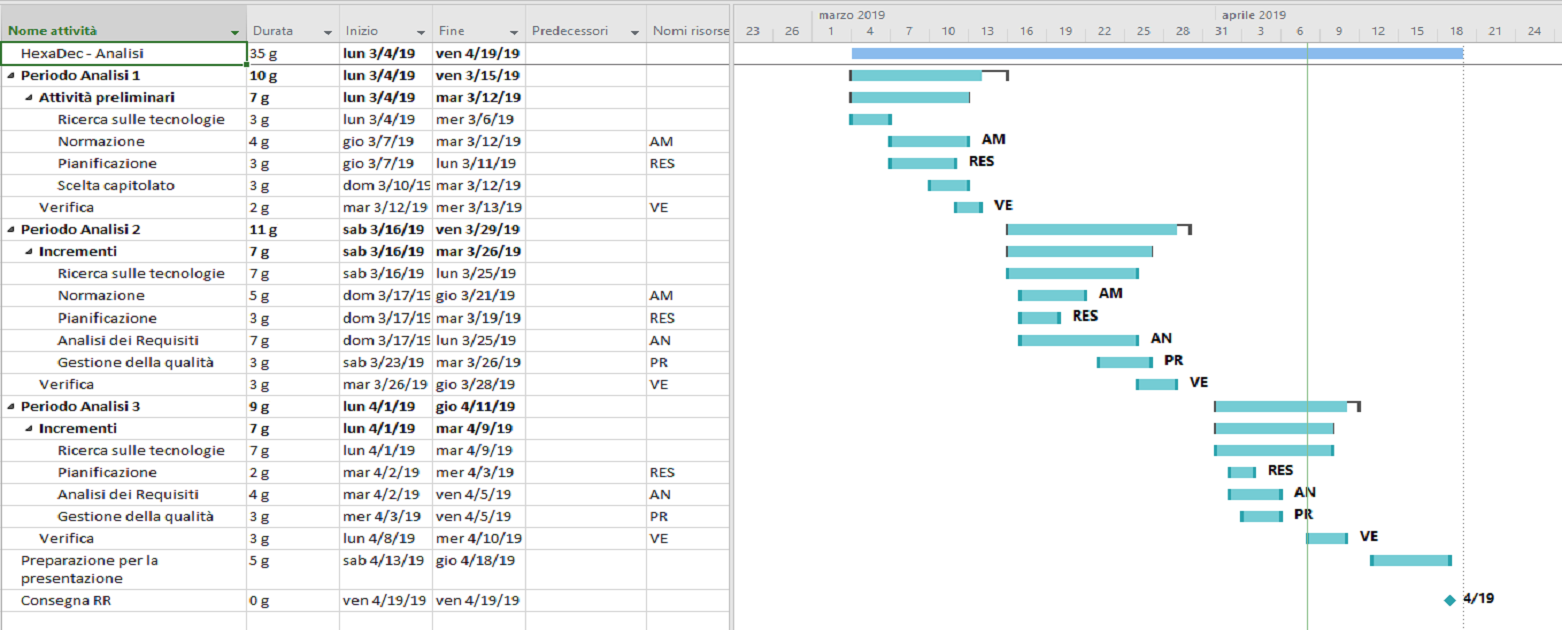
\includegraphics[width=\textwidth,height=\textheight,keepaspectratio]{immagini/gantt/GantRR.png}
                \caption{Diagramma di Gantt nella fase di \textit{Analisi}}
            \end{figure}
    
    \subsection{Progettazione architetturale}
    \textbf{Periodo}: dal 20-04-2019 al 17-05-2019. \newline
    Inizia al termine della fase di \textit{Analisi} e termina con la consegna della \RP.
    Questa fase si scompone in due periodi.

        \subsubsection{Periodo progettazione architetturale 1}
            \begin{itemize}
                \item Pianificazione: aggiustamenti alla pianificazione futura delle attività;
                \item Normazione: apporto modifiche alle norme secondo le indicazioni fornite dal docente;
                \item Analisi dei requisiti: apporto modifiche alla norme secondo le indicazioni fornite dal docente;
                \item Gestione qualità: apporto modifiche e/o aggiunte alle metodologie di qualità;
                \item Ricerca sulle tecnologie: aggiornamento degli strumenti utilizzati;
                \item Verifica.
            \end{itemize}
        
        \subsubsection{Periodo progettazione architetturale 2}
            \begin{itemize}
                \item Ricerca sulle tecnologie: studio di \glo{Amazon Lex}, \glo{DynamoDB}, \glo{Amazon Serverless}, \glo{Kotlin}, \glo{Node.js};
                \item Normazione;
                \item Pianificazione;
                \item Progettazione PoC: progettazione \glo{Proof of concept}(PoC), redazione della \glo{Technology Baseline} (TB);
                \item Codifica: scrittura codice per la PoC;
                \item Verifica;
                \item Presentazione.
            \end{itemize}

        \subsubsection{Diagramma di Gantt delle attività}
            \begin{figure}[H]
                \centering
                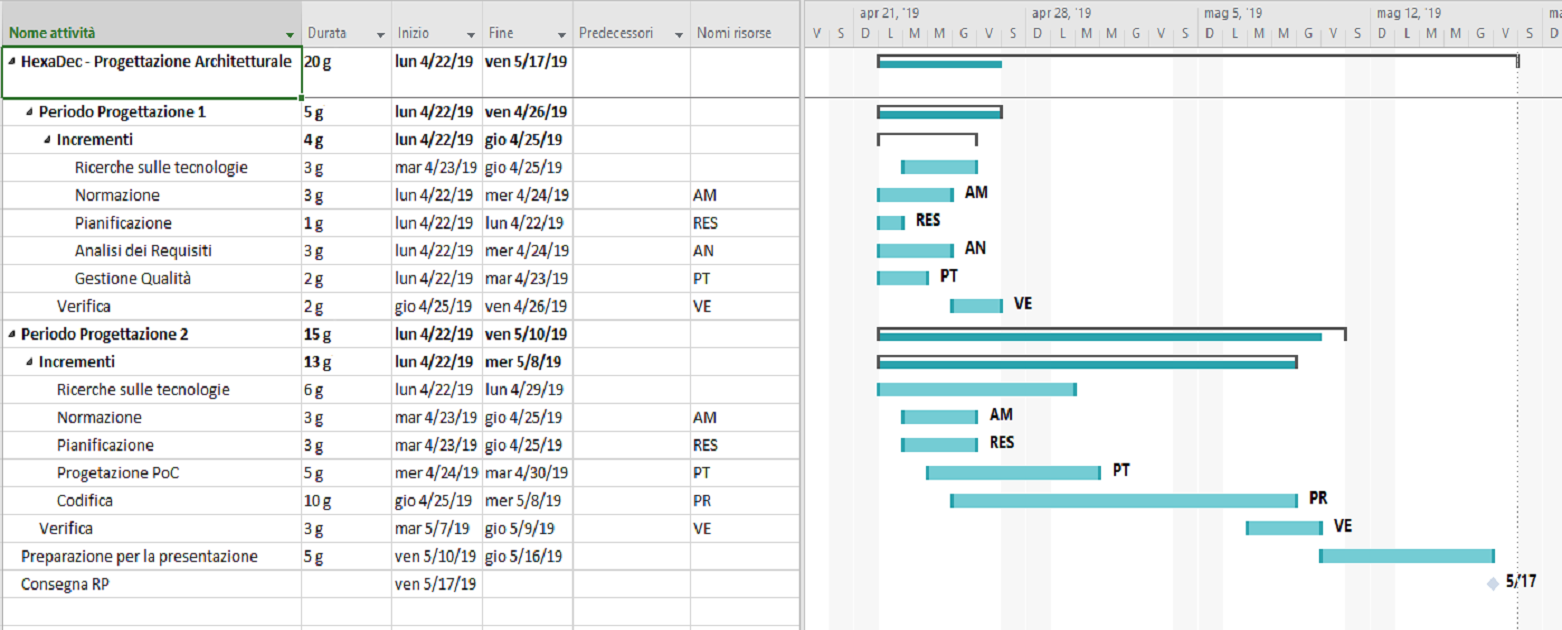
\includegraphics[width=\textwidth,height=\textheight,keepaspectratio]{immagini/gantt/GantRP.png}
                \caption{Diagramma di Gantt nella fase di \textit{Progettazione architetturale}}
            \end{figure}

    \subsection{Progettazione di dettaglio e codifica}
    \textbf{Periodo}: dal 18-05-2019 al 17-06-2019.  \newline
    Inizia al termine del periodo di \textit{Progettazione architetturale} e termina con \RQ.
    Questa fase si scompone in due periodi.
        \subsubsection{Periodo dettaglio e codifica 1}
            \begin{itemize}
                \item Normazione;
                \item Pianificazione: aggiustamenti alla pianificazione futura delle attività;
                \item Analisi dei Requisiti;
                \item Gestione qualità;
                \item Progettazione: miglioramento delle specifiche progettuali del PoC e sistemazione TB;
                \item Verifica.
            \end{itemize}
        
        \subsubsection{Periodo dettaglio e codifica 2}
            \begin{itemize}
                \item Normazione;
                \item Progettazione TB: miglioramento e incremento delle specifiche progettuali del PoC;
                \item Codifica: stesura codice con continue aggiunte di funzionalità per il primo rilascio;
                \item Manuale utente: produzione del documento \docNameMU{};
                \item Verifica: verifica dei documenti prodotti;
                \item Presentazione.
            \end{itemize}

    \subsubsection{Diagramma di Gantt delle attività}
            \begin{figure}[H]
                \centering
                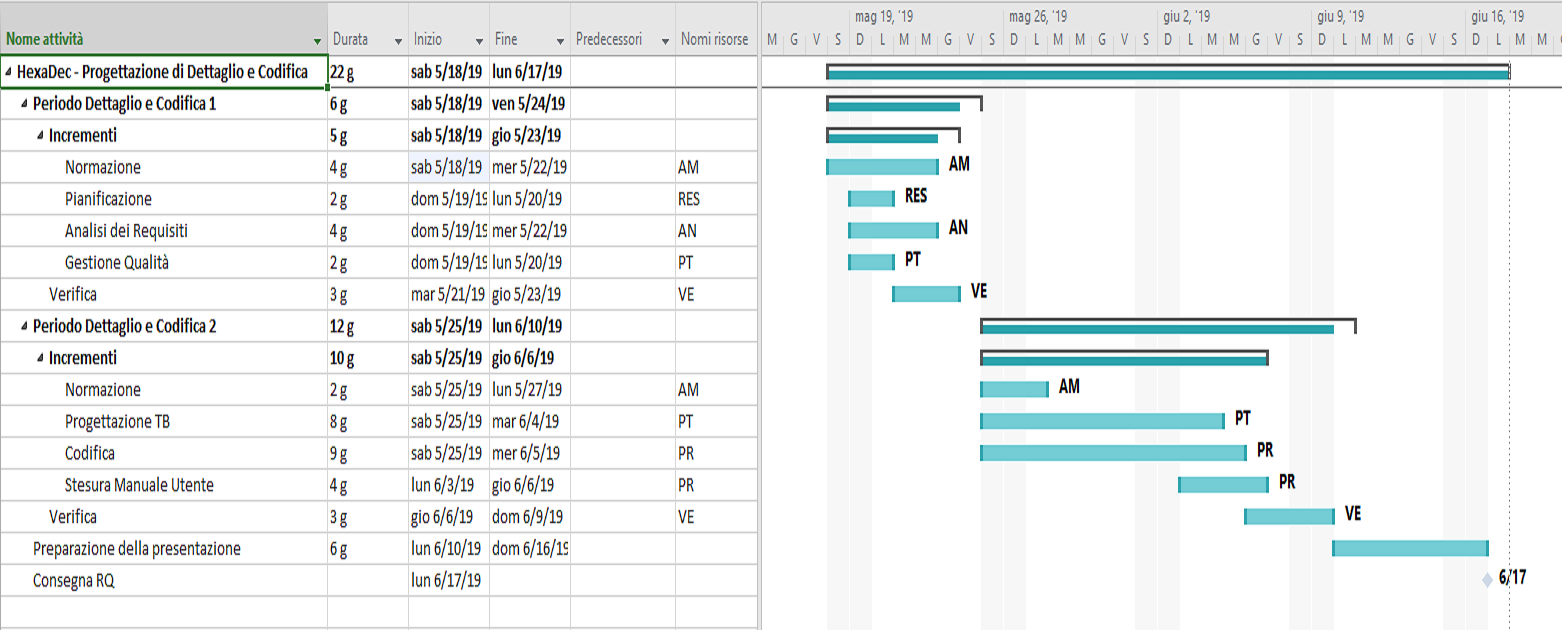
\includegraphics[width=\textwidth,height=\textheight,keepaspectratio]{immagini/gantt/GantRQ.png}
                \caption{Diagramma di Gantt nella fase di \textit{Progettazione di dettaglio e codifica}}
            \end{figure}

    \subsection{Validazione e collaudo}
    \textbf{Periodo}: dal 18-06-2019 al 15-07-2019.  \newline
    Inizia al termine del periodo di \textit{Progettazione di dettaglio e codifica} e termina con \RA.
    Questa fase si suddivide in due periodi.
        \subsubsection{Periodo collaudo 1}
            Sistemazione della documentazione:
            \begin{itemize}
                \item Normazione;
                \item Analisi dei requisiti;
                \item Gestione qualità;
                \item Pianificazione;
                \item Manuale utente.
            \end{itemize}
        
        \subsubsection{Periodo collaudo 2}
            \begin{itemize}
                \item Codifica: versione finale del prodotto;
                \item Manuale sviluppatore: produzione del documento \docNameMS;
                \item Validazione: test di qualifica e collaudo;
                \item Presentazione: preparazione per la revisione. 
            \end{itemize}
            
        \subsubsection{Diagramma di Gantt delle attività}
            \begin{figure}[H]
                \centering
                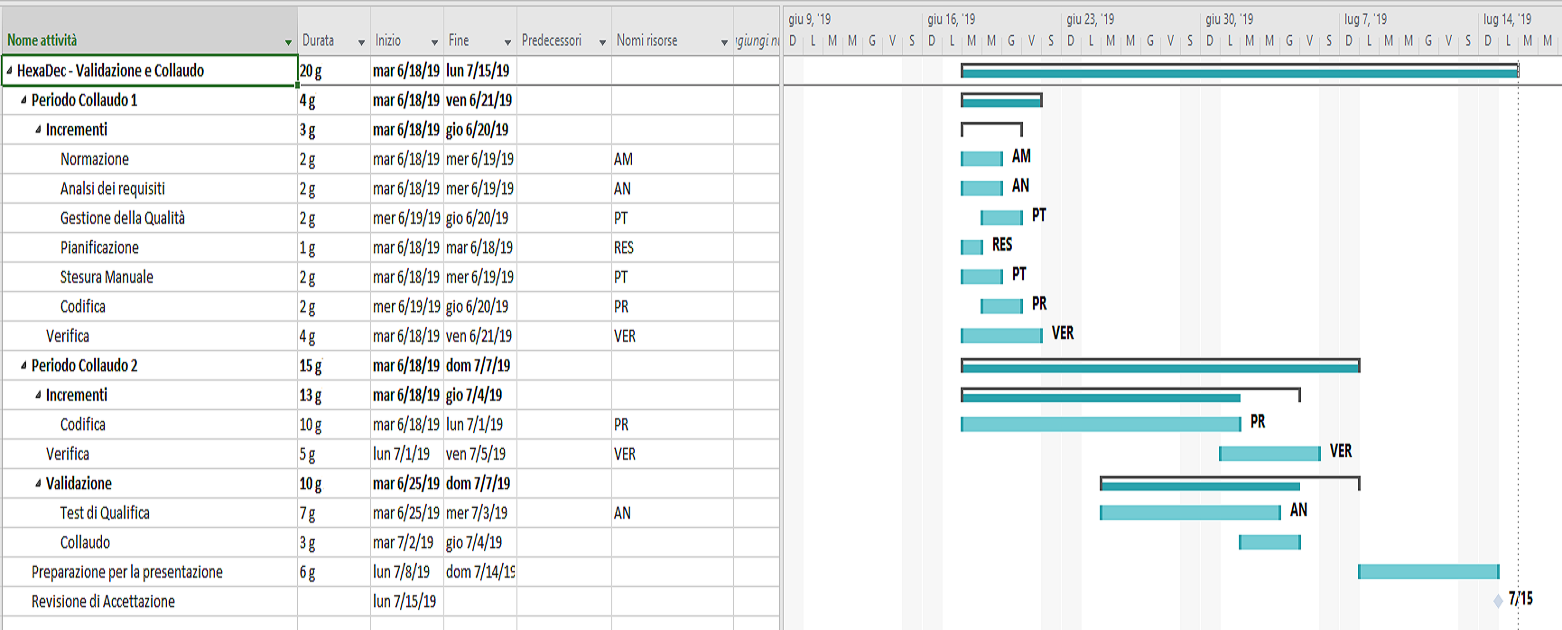
\includegraphics[width=\textwidth,height=\textheight,keepaspectratio]{immagini/gantt/GantRA.png}
                \caption{Diagramma di Gantt nella fase di \textit{Validazione e collaudo}}
            \end{figure}